\chapter{Analyse von Mrk 421 mit NAGIC STandardanalyse}
Sowohl die Programme zur Kalibration, als auch die Standard-Analyseprogramme sind im MARS (MAGIC Analysis and Reconstruction Software) -Paket enthalten.
Dieses Software Paket ist eine Sammlung an ROOT-Skripten und Macros.
In den folgenden Kapiteln werden die wichtigsten Programme zur Gamma-Hadron-Separation (Kapitel \ref{sec:GH-Separation}), Lichtkurven-Berechnung (Kapitel \ref{sec:Lichtkurve}) und Spektrumsrekonstruktion (Kapitel \ref{sec:Unfolding}) kurz erklärt.

Danach wird die Analyse der AGN durchgeführt.
Der Datensatz des gesamten Jahres 2012 wird in vier Teile geteilt und einzeln analysiert. 
In Abschnitt BLABLA werden dann alle Ergebnisse zu einer gesamten Lichtkurve zusammengefasst.


\section{Signal-Untergrund-Trennung und Energieschätzung}
\label{sec:GH-Separation}
\subsection{GH Separation}
Da das Signal-Untergrund-Verhältnis zwischen Gamma-Schauern aus der Quelle und hadronischen Schauern kleiner als 1\% ist (sogar für helle Quellen), werden gute Verfahren benötigt, um das Signal vom Untergrund zu trennen.
In der Standard-MAGIC-Analysekette übernimmt diese Aufgabe das Programm \texttt{Coach} und es wird zu diesem Zweck ein Random Forest genutzt. [siehe Breimann]
Dieser RF basiert auf einer Sammlung an Entscheidungsbäumen mit zufälligen Parametern in ihren Knoten.
Um einen solchen RF zu trainieren, benötigt man ein Trainingsset aus MCs und Untergrunddaten, von denen die Klassenzugehörigkeit (Signal oder Untergrund) genau bekannt ist.

Jedes Event wird durch die in Kapitel \ref{sec:Star-ImageCleaning} beschriebenen Imageparameter charakterisiert.
Im Ausgangsknoten ist das komplettes Sample mit allen Bildarametern.
Dieser Knoten wird dann in 2 Nachfolgeknoten geteilt, indem in einem Bildparameter geschnitten wird.
Beim Splitting Prozess werden die  Parameter für das Splitten zufällig aus einer vorher begrenzten Menge gezogen und der Parameter mit dem minimalen Gini-Index zum Splitten benutzt.
Mit Hilfe des Gini-Index kann die Ungleichheit der beiden Verteilungen als Funktion des Schnittes angegeben werden, der gerade angewendet wurde.
Ist der Gini-Index von einem Knoten null, so ist in diesem Knoten nur noch eine Klasse vorhanden.
% So bedeutet ein kleiner Gini-Koeffizient, dass die Verteilungen ähnlich sind und ein großer, dass sie ungleich sind. 

Dieses Splitten geschieht so lange bis die Anzahl der Events in einem Knoten zu gering wird, oder in einem Knoten nur noch eine Klasse vertreten ist.
In diesen Endknoten (terminal nodes) werden dann die Events mit einem Label (Gamma oder Hadron) versehen. 
Befindet sich in einem Endknoten noch eine Mischung beider Klassen, wird ein Mittelwert vergeben.
So folgt jedes Event einem Pfad durch die i verschiedenen Bäume und wird von allen klassifiziert.
Danach wird ihm ein finales Label, die hadroness, zugewiesen:

\begin{equation}
 h(Event)=\frac{ \sum_{i=1} ^{n_{trees}} l_i(Event)}{n_{trees}}
\end{equation}



\subsection{Energierekonstruktion mit Hilfe von Look up Tables}
Die Energie der Primärteilchen ist proportional zur Anzahl der Cherenkovphotonen im Schauer und so zum Parameter \texttt{size}.
Allerdings ist \texttt{size} abhängig vom Zenitwinkel, der Lage des Schauers in der Kamera, dem Impact-Parameter und der Höhe des Schauermaximums.
Beruhend auf dieser Tatsache wird nun eine Tabelle erstellt.
Das MC Trainingsset wird nun in Bins für jeden Parameter, der für die Energierekonstruktion benutzt werden soll, aufgeteilt.
So wird eine mehrdimensionale Tabelle mit der Energie der MC Events, die zu jedem Bin gehört, erstellt.
Den realen Daten wird dann anhand ihrer Parameter das passende Energiebin in der Tabelle zugeteilt und so eine estimated Energy zugeordnet.


\subsection{Position Reconstruction}
Ziel ist es, die Herkunft des Primärteilchens zu rekonstruieren. 
Der Abstand zwischen dem Schauerschwerpunkt und der Quellposition auf der Hauptachse in der Kamera wird mit dem Parameter \texttt{Disp} bezeichnet.
Es gibt zwei Möglichkeiten, diesen Parameter zu rekonstruieren: Zum Einen sind dies Ghostbusting-Methoden, die die Asymmetrie der Schauer benutzen oder aber RF.

Wird mit zwei Teleskopen observiert, ist die Disp-Rekonstruktion einfacher.
Wie in Abb.\ref{Disp} zu sehen ist, ist perfektes Ghostbusting möglich.

\begin{figure}
    \centering
    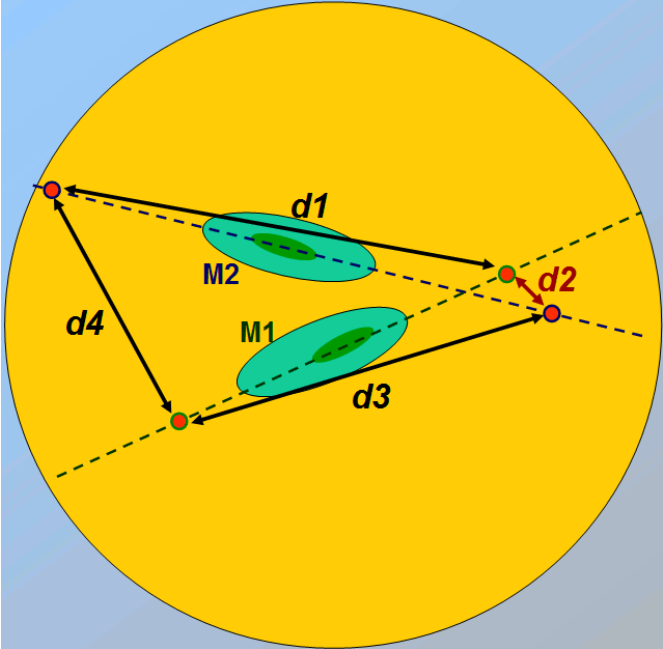
\includegraphics[width=0.5\textwidth]{./Plots/04_MrkAnalyse/Disp.png}
    \caption{Rekonstruktion des Parameters \texttt{Disp}}
    \label{Disp}
\end{figure}

Nur eine der beiden möglichken Quellpositionen ist kompatibel mit dem anderen Teleskop und so ist die bevorzugte Position der Quelle die, die näher am Schnittpunkt der beiden Hauptachsen liegt und damit ist dann der Parameter \texttt{Disp} eindeutig bestimmt.



\section{Berechnung der Lichtkurve}
\label{sec:Lichtkurve}
Der Gamma-Fluss, d.h. die Rate der  Gammateilchen pro Einheitsfläche ist Ausgangsgröße für die Lichtkurve:

\begin{equation}
 \Phi=\frac{d^2 N}{dS dt}. 
\end{equation}

Dafür wird die Anzahl der detektierten Gammas, die effektive Observationszeit und die effektive Fläche des Detektors benötigt.
Nach der Energie differenziert ist diese Größe der differentielle Fluss pro Energie:

\begin{equation}
 \frac{d\Phi}{dE}=\frac{d^3N}{dSdtdE},
\end{equation}

bzw. der integrale Fluss:
\begin{equation}
 \Phi_{E>500GeV}=\int_{500GeV}^{\infty}\frac{d\Phi}{dE}dE.
\end{equation}


Die zeitliche Entwicklung des integralen Flusses wird nun Lichtkurve genannt.
Das Binning kann nach Lust und Laune gewählt werden.
% , tageweise oder minutenweise... Je nachdem, ob gerade irgendwas spannendes passiert (Flares oder so).

\subsection{Anzahl der exzess gammas}
Um die Anzahl der Gammateilchen aus der Quelle zu bestimmen, wird ein $\theta^2$-Histogramm benutzt.
Dies ist ein Histogramm der quadrierten Entfernungen zwischen der rekonstruierten Quellposition und der nominalen Quellposition.
Gammas aus der Quelle haben ein kleineres theta während der Background eine annähernd flache Verteilung liefert. 

\begin{figure}
    \centering
    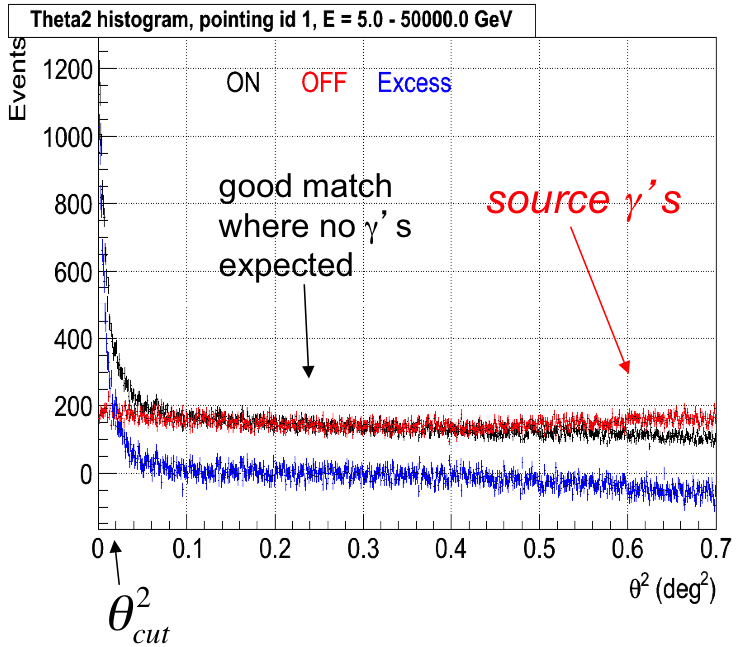
\includegraphics[width=0.8\textwidth]{./Plots/04_MrkAnalyse/Theta2Example.png}
    \caption{$\theta^2$-Verteilung... blabla}
    \label{Disp}
\end{figure}
% BILDBILDBILD (abelardos talk in zeuthen, der auf der flute seite verlinkt ist)

Um die Anzahl der wirklich Exzess-Events zu kriegen, müssen von den Events aus der Quellrichtung noch die Background Events abgezogen werden und es wird meist noch ein Schnitt in $\theta^2$ gemacht.

Die Beobachtungsmethode von MAGIC ist die Wobble-Beobachtung, d.h. das Teleskop ist nicht direkt auf die Quelle ausgerichtet, sondern einen kleinen Winkel daneben.
Dank der alt-azimutalen Montierung rotiert die Quelle um das Zentrum in der Kamera und es ist möglich einen Punkt gegenüber der Quelle als Off-Position zu benutzen.
Vorteil dieser Methode ist, dass es keine separate Off-Datennahme geben muss.
Allerdings tauchen so die Quellgammas auch in der Off-$\theta^2$-Verteilung auf, haben aber ein großes $\theta^2$.
Eine Off-Position, die zu nahe an der Quelle ist, ist nicht zu empfehlen.

\subsection{Effektive On Zeit}
Die effektive On-Time berücksichtigt die Totzeit in der Datennahme.
Abhängig vom Chip ist die Totzeit bei den aktuellen Chips bei 26$\mu$s.

\subsection{Effektive Fläche}
Als effektive Fläche wird die Fläche am Boden, die orthogonal zur Herkunftsrichtung der Schauerteilchen ist, bezeichnet.
Die Größe dieser effektiven Fläche ist abhängig von der Energie und dem Zenitwinkel des Schauers.
In MARS wird diese Größe mit Hilfe von MCs folgendermaßen berechnet:

\begin{equation}
 A_{eff}(E)=\frac{N_{\gamma, final}}{N_{\gamma, simulated}}A_{MC, total}
\end{equation}

Dafür wird eine bestimmte Anzahl an Gammas ($N_{\gamma, simulated}$) auf einer uniformen Fläche $A_{MC,total}$ simuliert. 
Die Größe $N_{\gamma, final}$ ist die Anzahl der Gammas, die das Cleaning und alle Cuts überlebt hat.


\section{Entfaltung des Energiespektrumpfs}
\label{sec:Unfolding}
Bei der Messung mit IACTs handelt es sich um eine indirekte Messung.
Die Energie des Schauer-auslösenden Teilchens ist nicht direkt messbar.
Die Bildparameter und damit auch die geschätzte Energie $E_{est}$ haben eine begrenzte Auflösung und erfordern die Methode der Entfaltung.

Die Probleme, die bei der Messung auftreten sind:

\begin{itemize}
 \item Begrenzte Akzeptanz: Nicht alle Schauer, die ein Teilchen auslöst können vom Teleskop detektiert werden.
 \item Indirekte Messung: Da eine direkte Messung nicht möglich ist, wird anhand von gemessenen Parametern, wie der Größe des Schauers in der Kamera etwa, mit Hilfe eines RF die Energie geschätzt.
       Die Vorraussetzung dafür ist, dass diese in echt gemessenen Parameter stark mit der Energie korrelliert sind.
 \item Begrenzte Auflösung: Es ist nur möglich mit begrenzter Genauigkeit aus den Bildparametern die Energie zu rekonstruieren, d.h. es existiert eine Migration von Events.
       Wird die geschätzte Energie gegen die reale Energie aufgetragen, erhält man eine verschmierte Diagonale (siehe Abb.\ref{EnergyEst_EnergyTrue})
\end{itemize}

\begin{figure}
    \centering
    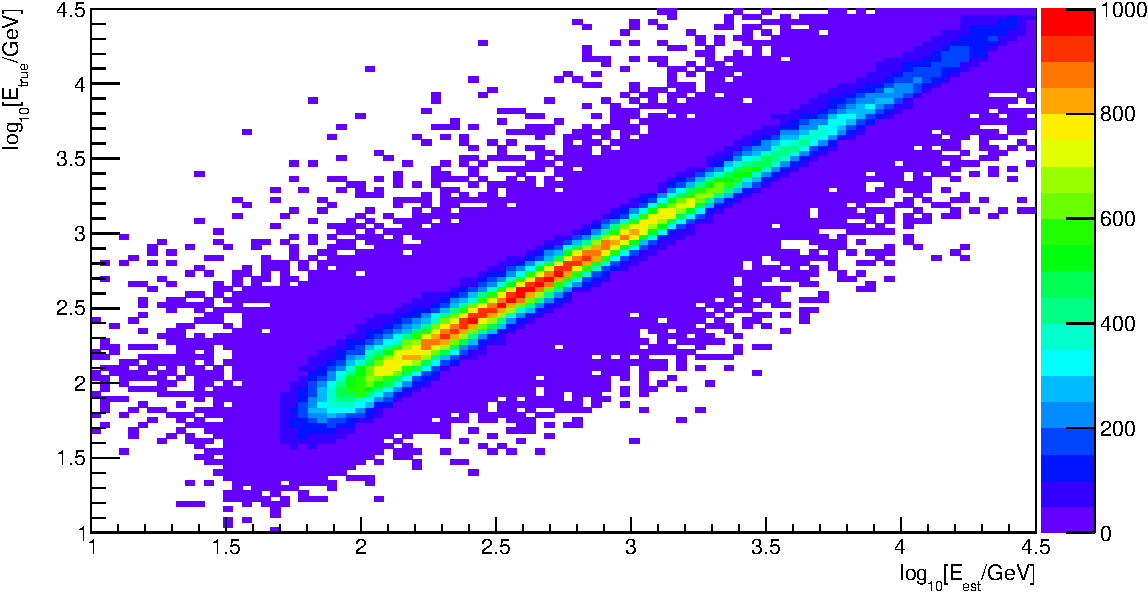
\includegraphics[width=0.8\textwidth]{./Plots/04_MrkAnalyse/EnergyEst_EnergyTrue.pdf}
    \caption{Estimated Energy gegen True Energy.}
    \label{EnergyEst_EnergyTrue}
\end{figure}

Durch die Methode der Entfaltung können diese Probleme berücksichtigt werden und das Problem lässt sich mit einer Fredholmschen Integralgleichung darstellen:

\begin{equation}
 g(y)= \int_c^d M(x,y) f(x) dx + b(y)
\end{equation}
\begin{centering}
  \tiny{mit g(y): gemessene Verteilung, f(x): gesuchte Verteilung, M(x,y): Migrationsmatrix bestimmt auf MCs, b(y): Background-Verteilung}
 \end{centering}

Diese Gleichung lässt sich auch bin-Weise darstellen:

\begin{equation}
 g_i=\sum_j M_{ij}f_j+b_i,
\end{equation}

wobei $M_{ij}$ nun die Wahrscheinlichkeit ist, dass ein Event in bin j in bin i gezählt wird.

Das Ziel der Entfaltung ist nun die wahre Verteilung $f$ zu finden.
Die Kovarianzmatrix der gesuchten Verteilung ergibt sich dann mit der Kovarianzmatrix der gemessenen Verteilung zu:

\begin{equation}
 \mathbf{V[f]}=\mathbf{M}^{-1}\mathbf{V[g]}\mathbf{(M}^{-1})^T
\end{equation}

Da die Invertierung der Migrationsmatrix oft zu oszillierenden Lösungen führt, versucht man die Methode der kleinsten Quadrate.

\begin{equation}
 \chi_0^2=(\vec{g}-\mathbf{M}\vec{f})^T \mathbf{V}^{-1}[\vec{g}](\vec{g}-\mathbf{M}vec{f}).
\end{equation}

Dies gilt nur für Gaussverteilte Daten, also nicht für Bins mit kleinen Eventszahlen.
Für diese muss nun die Poisson-Statistik benutzt werden und der Log-Likelihood-Ausdruck minimiert werden:

\begin{equation}
 L_0(a)=\sum_i (g_i(a)-g_{i,m}\cdot \ln g_i(a)).
\end{equation}

Außerdem ist es nötig, eine Regularisierung einzuführen, um die kleinen Ausdrücke in der Migrationsmatrix, die während der Entfaltung verstärkt werden, zu unterdrücken.
Durch Einführung eines Regularisierungsterms werden Anforderungen an die Lösung gestellt, bei zu doller Regularisierung aber auch ein Bias eingeführt.

Im Allgemeinen wird Regularisierung durch Addition eines Regularisierungsterms gemacht, sodass:

\begin{equation}
 \chi^2=\chi_0^2 +\frac{\tau}{2} Reg(f).
\end{equation}

Verschiedene Arten der Regularisierung können in der Analyse gewählt werden.
Es ist ebenfalls möglich, eine Vorwärtsfaltung durchzuführen, wobei ein bestimmtes Modell als Annahme gewählt wird und freie Parameter dieses Modells bestimmt werden.
Zum Testen ist dies eine gute Alternative, allerdings keine richtige Entfaltung, da das Ergebnis Modellabhängig bleibt.

\section{MrK421 Analyse}
In diesem Abschnitt wird die Analyse der Daten beschrieben, wobei für jede der vier Datenepochen sowohl Lichtkurve als auch Spektrum gezeigt werden.
Dabei wird die Analyse des zweiten Teils der Daten exemplarisch für die Stereo-Analyse erklärt ABSCHNITT BLABLA, während die anderen Zeitabschnitte des Jahres mit stereoskopischer Beobachtung ABSCHNITT BLA UND BLA analog ausgewertet werden.
Auf die Mono-Datennanalyse wird in section BLABLA danach eingegangen.
Zusammenfassend wird noch eine Lichtkurve aller Daten gezeigt.


\subsection{Überblick über die Daten}
Die Daten, die mir zur Verfügung standen, sind Daten der Quelle Mrk421, die 2012 genommen wurden.
Die Daten gliedern sich so folgendermaßen:

\begin{itemize}
 \item Datenset 1: 2012-02-25 - 2012-02-29
 \item Datenset 2: 2012-03-18 - 2012-04-27
 \item Datenset 3: 2012-05-23 - 2012-06-19
 \item Datenset 4: 2012-12-11 - 2012-12-23
\end{itemize}

Datenset 1 und Datenset 2 unterscheiden sich in ihrer PSF, weswegen zwei verschiedene MC-Sets verwendet werden.
In beiden Zeitbereichen war eine Stereobeobachtung mit beiden Teleskopen möglich.

Beim 3. Datenset handelt es sich um Mono-Daten. 
Aufgrund der kaputten MAGIC I - Kamera und der geplanten Upgrade-Pause, wurden nur MAGIC II betrieben.

Im 4. Datenset war das Upgrade abgeschlossen und die alte MAGIC I Kamera durch eine neue Kamera ersetzt und es wurden wieder Stereobeobachtungen durchgeführt.
Aufgrund der Hardware-Veränderungen und einer anderen PSF wurden wieder neue MCs produziert.

Die Analyse des ersten Teils der Daten befindet sich in Kapitel BLA und die des zweiten Teils in Kapitel BLABLA.
Danach erfolgt die dritte Analyseperiode mit Stereobeobachtungen in Kapitel BLA.
Die Mono-Analyse wird in Kapitel HORST beschrieben.


\subsection{Datenset 2}
Anhand der genommenen Mrk421 - Daten zwischen dem 18.3.2012 und dem 27.4.2012 wird nun die Analyse erklärt.
Diese Daten wurden unter einem Zenitwinkel von bis zu 30° genommen (siehe Abb.\ref{Datenset2_fZD}).

\begin{figure}
    \centering
    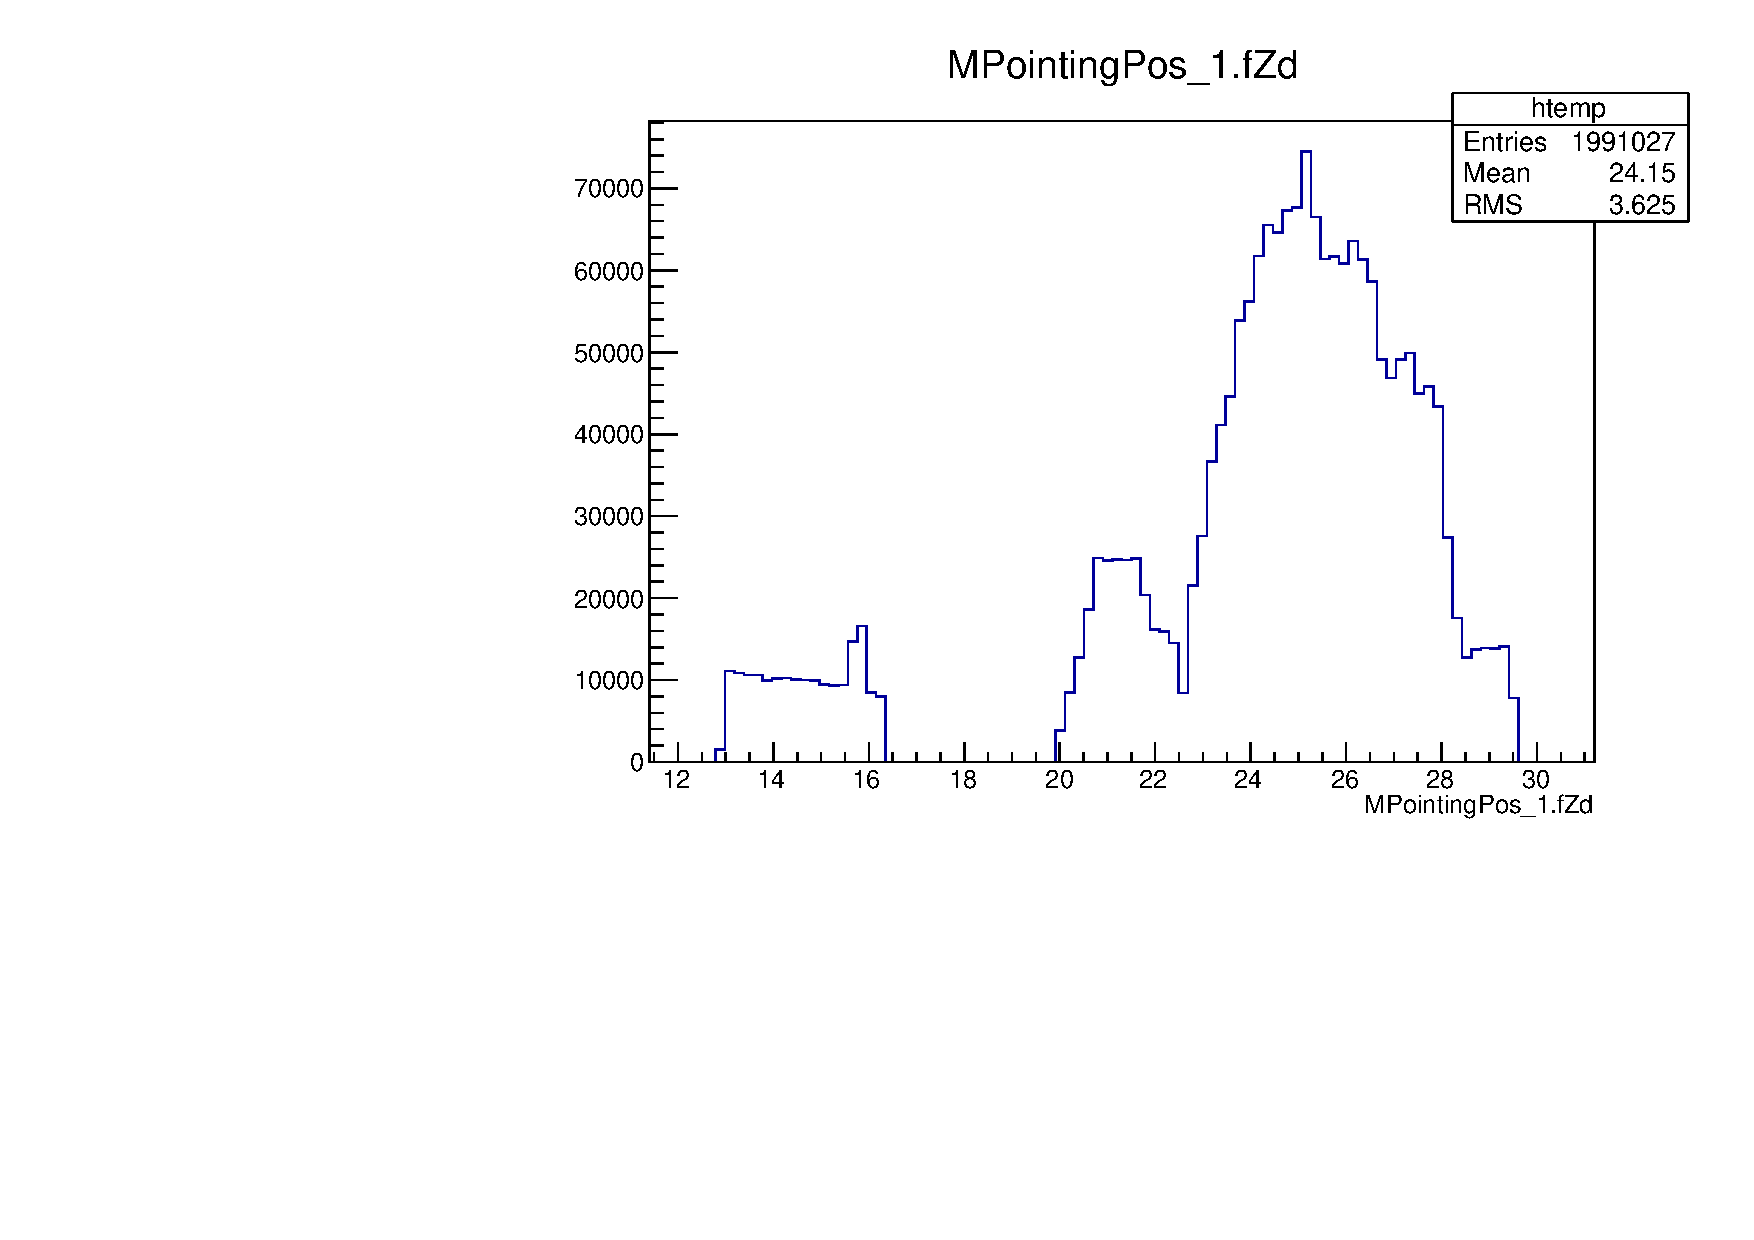
\includegraphics[width=0.6\textwidth]{./Plots/04_MrkAnalyse/Datenset2/Mrk421_Part2.pdf}
    \caption{Zenitverteilung der genommenen Daten.}
    \label{Datenset2_fZD}
\end{figure}


Da dieser Datensatz die meisten Daten beinhaltet, wird die Analyse examplarisch und ausführlich hieran durchgeführt.

Als Off-Daten dienen Daten anderer Quellen, welche in der gleichen Zeitspanne wie die zu analysierende liegen.

Mit Hilfe von Crab-Daten werden die Einstellungen für die Lichtkurvenbestimmung und Spektrumsrekonstruktion gesucht, da Crab einen bekannten stabilen Fluss hat. 


\subsubsection{Data-/Off-Data-/MC-/Crab-Selection und Qualitätsmerkmale}
Zunächst werden die Daten in diesem Zeitraum einem Datencheck unterzogen und die Daten herauszufiltern, die bei dunklen Bedingungen genommen wurden. 

Dafür wurde zunächst ein Cut im DC (MI < 500, M II < 800) durchgeführt.
Danach wurden mit Hilfe des MARS Macros \textit{Quate} alle Daten mit einem Zenitwinkel < 35° ausgewählt, Runs mit einer Länge unter 10s und Runs mit einer Abweichung des Pointing von 15arcmin verworfen.
Außerdem wurden die Mittelwerte der Parameter Rate, Number of Islands, Concentration, Width, Length gebildet und ebenfalls Ausreißer aussortiert um eine gute Qualität der Daten zu gewährleisten.

Diese Kriterien für den Datencheck wurden für die Mrk421-Daten, die Crab-Daten und die Off-Daten angewendet.

In der Tabelle \ref{tab:Datenset2} ist aufgelistet, welche Daten nach der Datenauswahl für die Analyse zur Verfügung stehen.


\begin{table}[!h]
\centering
\caption{Daten nach Datencheck}
\label{tab:Datenset2}
\begin{tabular}{lc}
  \toprule
  Quelle & nachm Datencheck übbere Zeit\\
  \midrule
  \midrule
  Mrk421 & 319min\\
  \midrule
  Crab & 400min\\
  \midrule
  0FGLJ0631 & 113min \\
  1ES1011 & 363min \\
  1ES1426 & 428min \\
  PG1553 & 1022min \\
  PKS1222 & 277min \\
  SegueJ & 3414min \\
  \bottomrule
  \bottomrule
\end{tabular}
\end{table}

Für diesen Teil der Analyse wurden die in Dortmund produzierten Standard-MC-Daten im Zenitbereich 5-35° genommen, in deren Simulation die alte MAGIC I Kamera simuliert wurde, allerdings schon der neue DRS4-Chip benutzt wurde.
Die PSF für MAGIC I ist 10.5 und die Mirror Fraction 0.58, während diese Werte für MAGIC II 10.2mm und 0.70 sind.

Es ist zu beachten, dass für alle Daten (Mrk 421/Crab/Off) und die MCs das gleiche Cleaning benutzt wird, da zu dieser Zeit zwei verschiedene Cleaning-Schwellen im Next-Neighbor-Cleaning gebräuchlich waren.
Die Core und Neighbor-Schwelle beträgt in diesen Daten 6, bzw. 3.


\subsubsection{Coach und Melibea}
Für das Training des RF für die GH-Separation und die Disp-Estimation ist es wichtig, dass in jedem Zenitbin genug Background-Daten vorhanden sind.
Wie in Abb.\ref{Datenset2_Zenitverteilung_Off} ist das gegeben.

\begin{figure}
    \centering
    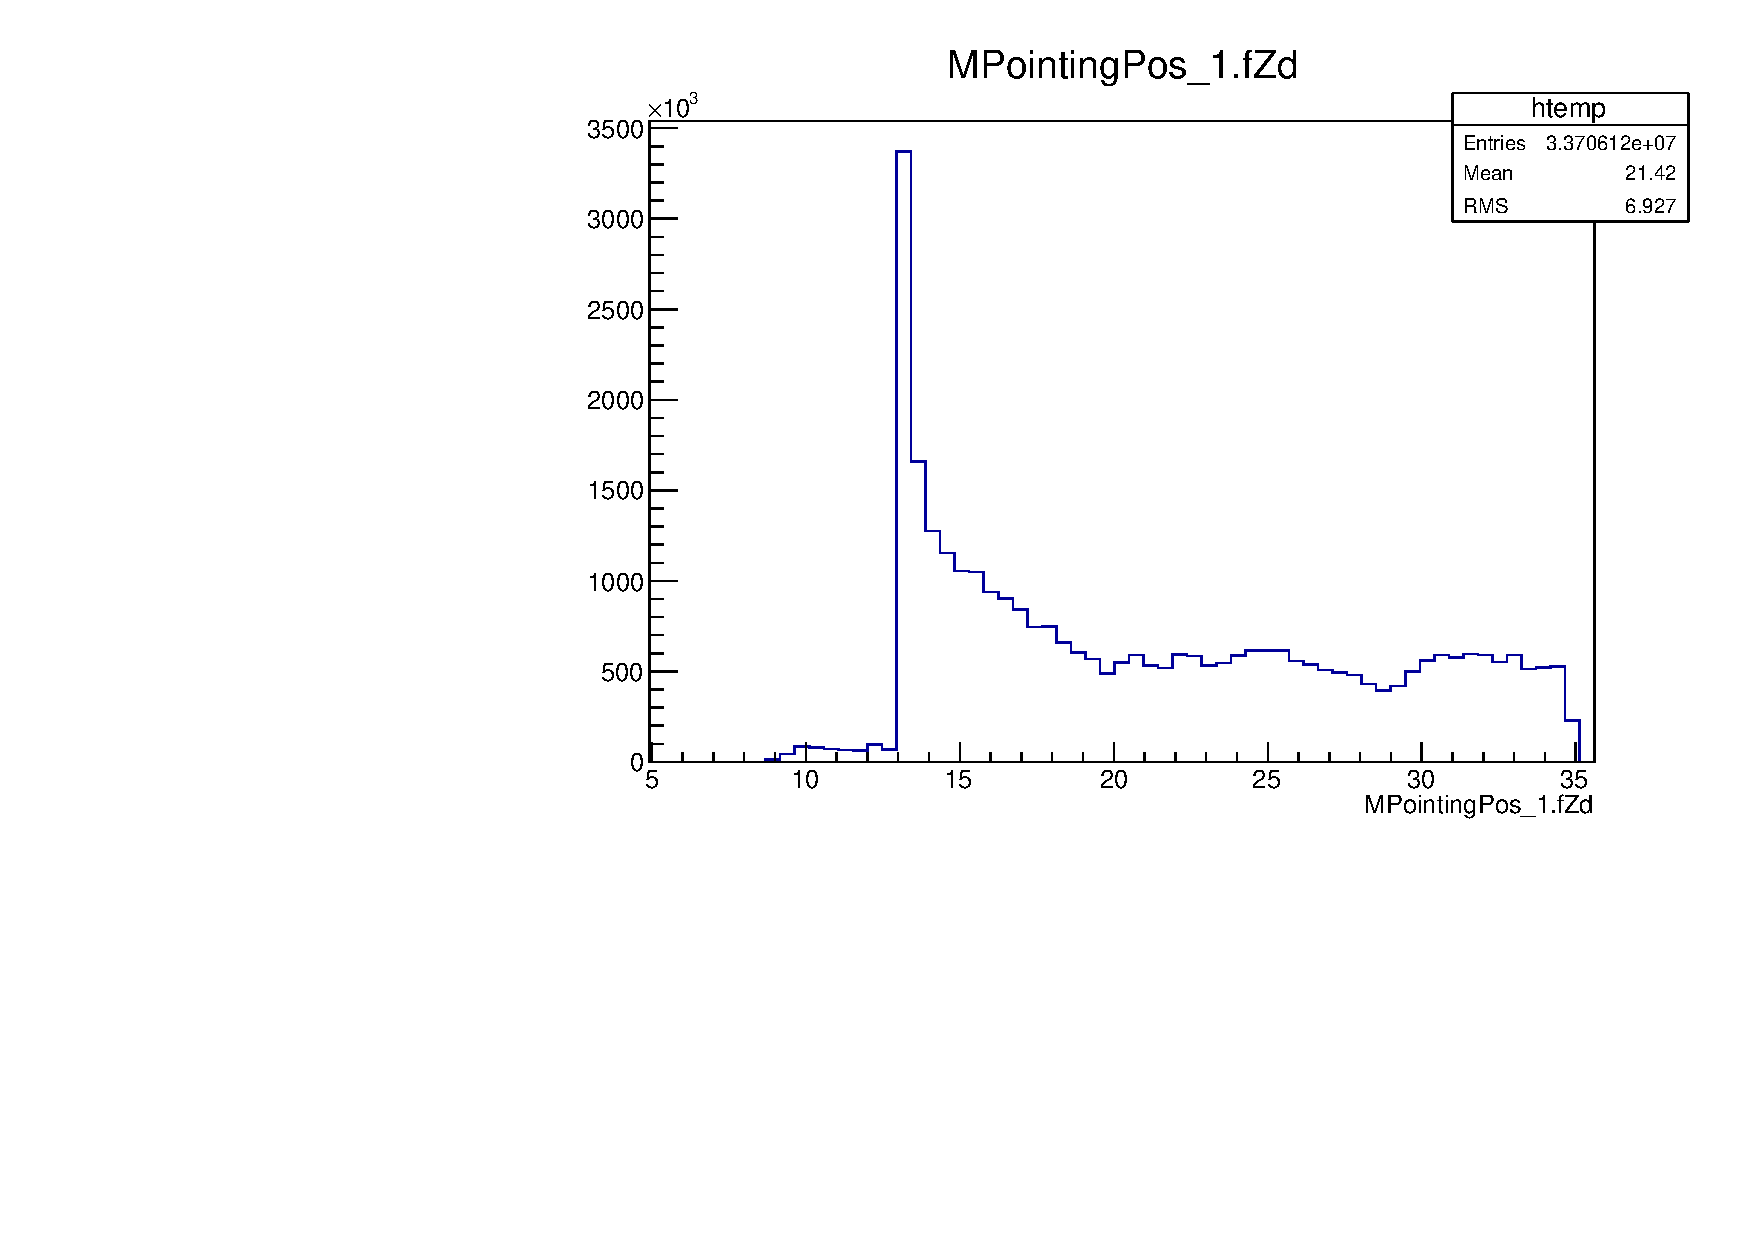
\includegraphics[width=0.6\textwidth]{./Plots/04_MrkAnalyse/Datenset2/Part2_2_Background_Zenith.pdf}
    \caption{Zenitverteilung der Off-Daten.}
    \label{Datenset2_Zenitverteilung_Off}
\end{figure}

Der MC-Datensatz wird nun in zwei Teile geteilt.
Der eine Teil, das Trainings-Set, wird zusammen mit den Off-Daten zum Trainieren des RF für die GH-Separtion und für Disp benutzt, sowie zum Aufstellen der Look Up Tables für die Energie.

Sobald Coach beendet ist, werden in Melibea die Daten nach Gamma- und Hadron-Events klassifiziert und jedem Event eine geschätzte Energie und ein Disp-Wert zugeordnet.
Das gleiche geschieht auch mit den Crab-Daten und dem anderen Teil der MCs, dem Test-Set.


\subsubsection{Lichtkurve von Crab}
Wie in Kapitel \ref{sec:Lichtkurve} beschrieben, wird nun sowohl für die Crab-Daten als auch für die Mrk421 Daten eine Lichtkurve erstellt.
Mit Hilfe der Crab-Daten werden die passenden Parameter (Hadroneffizienz und Theta-Quadrat-Effizienz) für die Lichtkurven-Bestimmung für Mrk421 ausgewählt.

Wie in Abb.\ref{Datenset2_Flute_Plots_Crab} zu sehen, ist es möglich mit Flute neben der Lichtkurve (vgl. Abb.\ref{Datenset2_LC_Crab}) auch noch einen Theta Quadrat Plot (vgl. Abb.\ref{Datenset2_theta^2_Crab}), sowie die spektrale Energie-Verteilung (vgl. Abb.\ref{Datenset2_SED_Crab}) zu berechnen.

\begin{figure}
  %-----------------------------Figure 1--------------------------------------------------------%
  \begin{subfigure}{0.45\linewidth}
  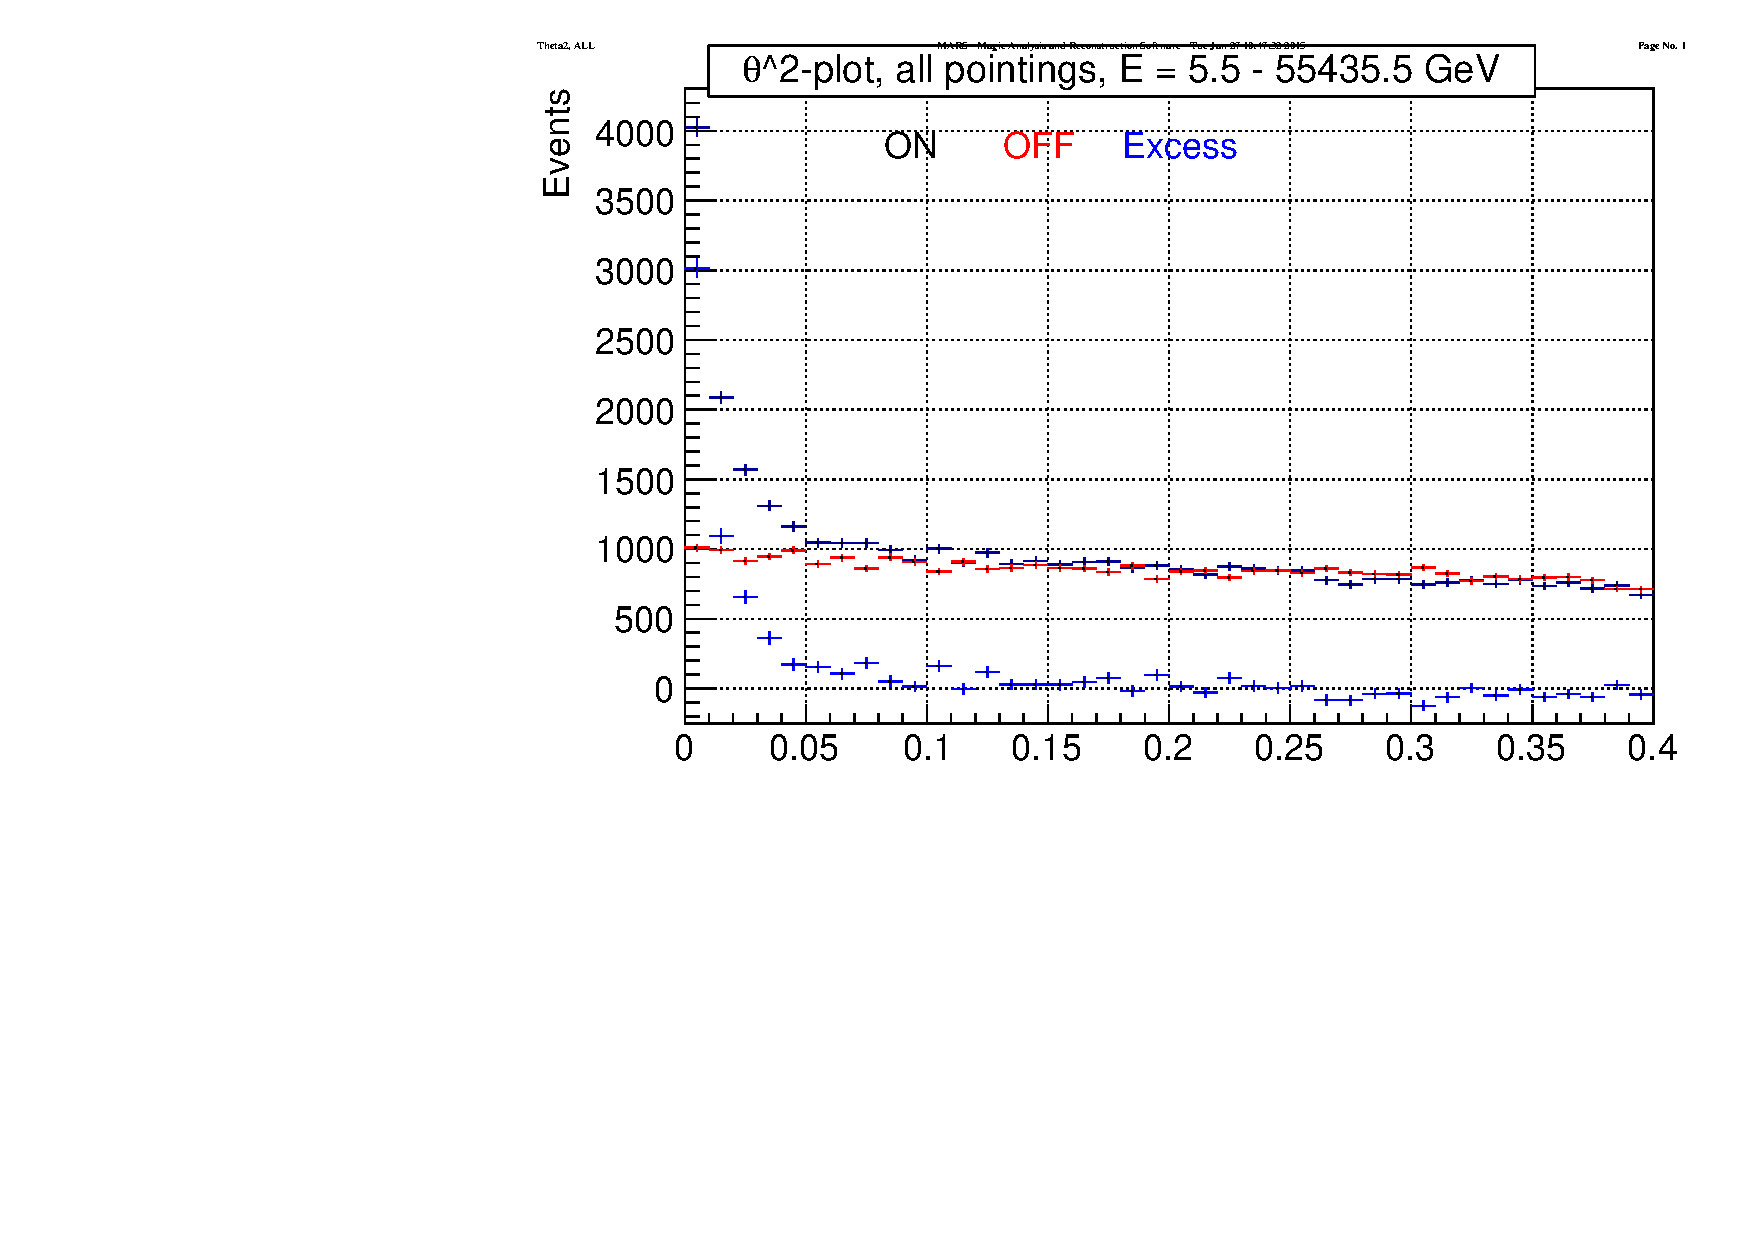
\includegraphics[width=\textwidth]{./Plots/04_MrkAnalyse/Datenset2/Theta_Quadrat.pdf}
  \caption{$\theta^2$-Plot für Crab}
  \label{Datenset2_theta^2_Crab}
  \end{subfigure}
  \hfill
  %-----------------------------Figure 2--------------------------------------------------------%
  \begin{subfigure}{0.45\linewidth}
  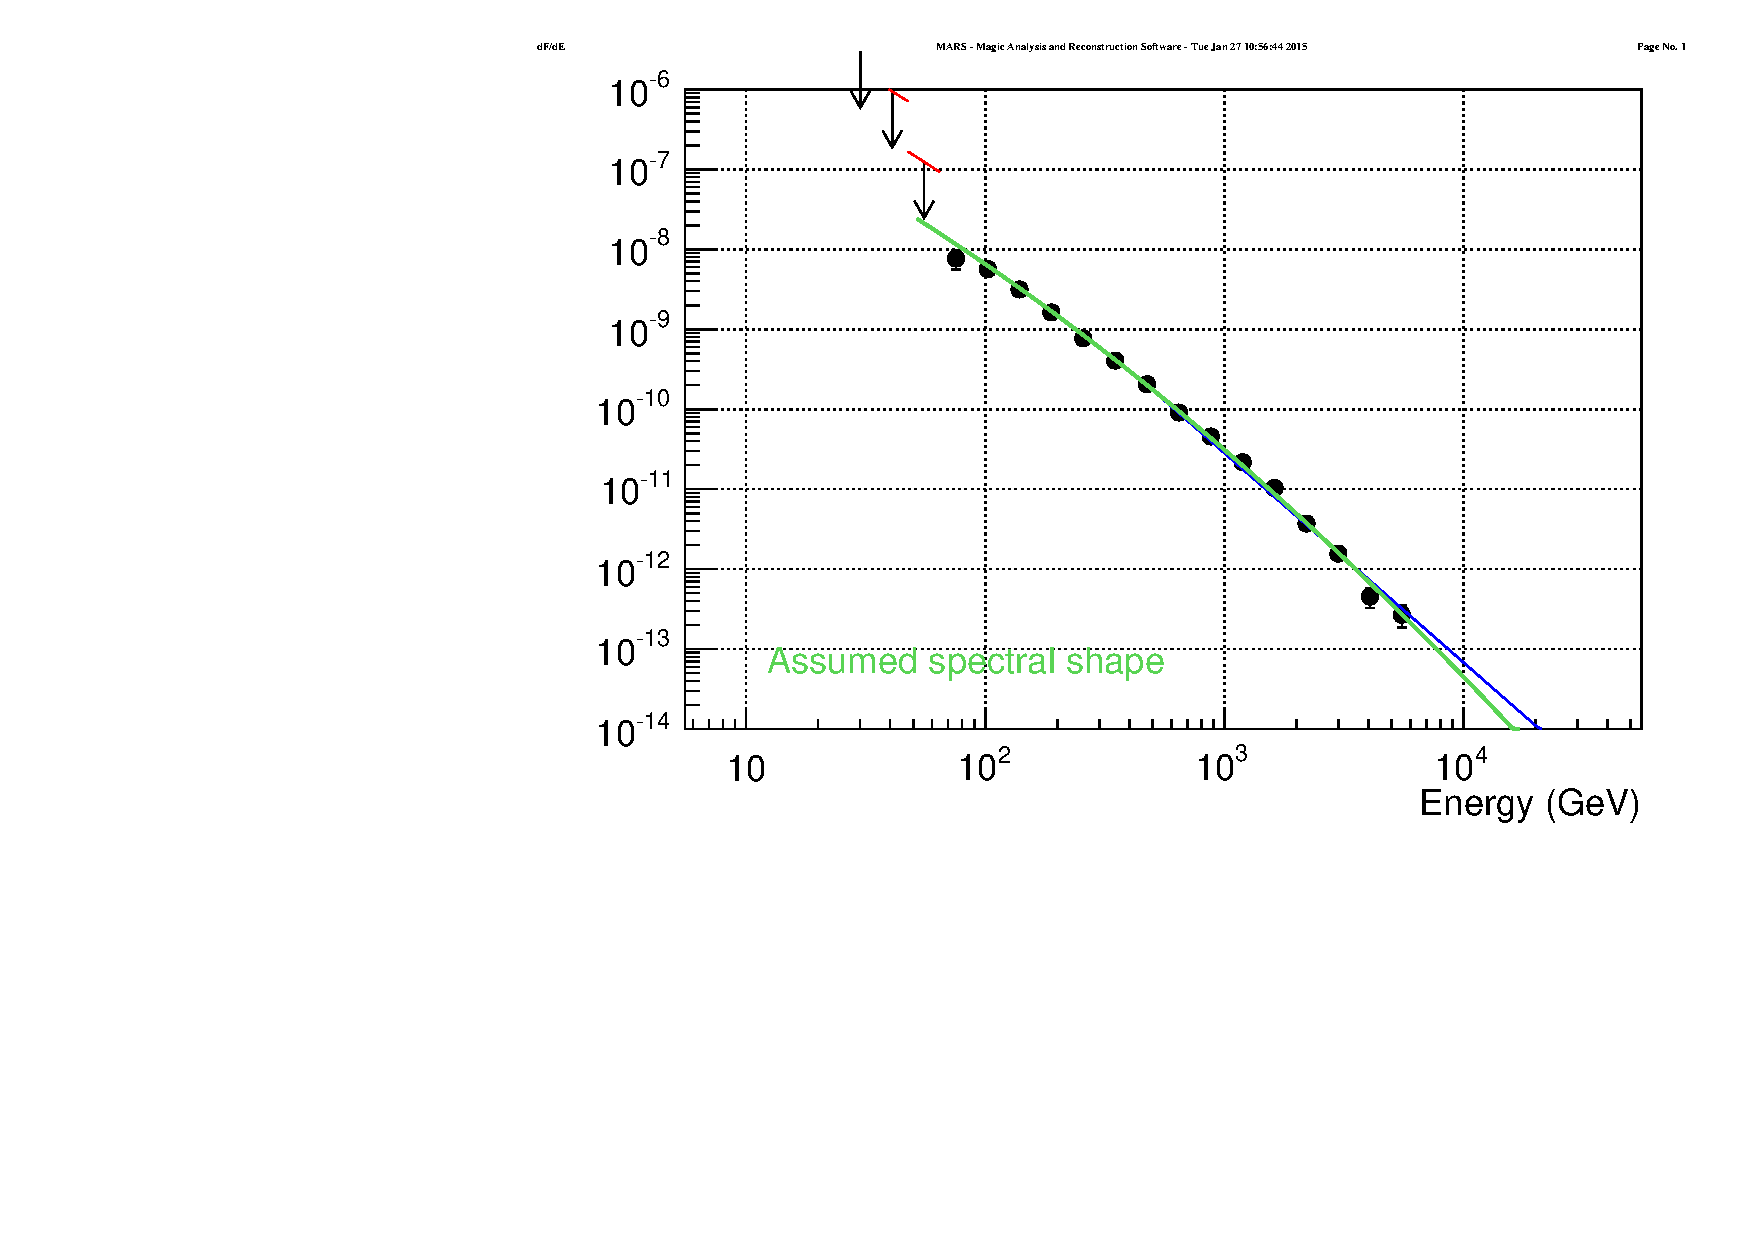
\includegraphics[width=\textwidth]{./Plots/04_MrkAnalyse/Datenset2/SpectralShape.pdf}
  \caption{Spectral Shape Crab}
  \label{Datenset2_SpectralShape_Crab}
  \end{subfigure}
  \hfill
  %-----------------------------Figure 3--------------------------------------------------------%
  \begin{subfigure}{0.45\linewidth}
  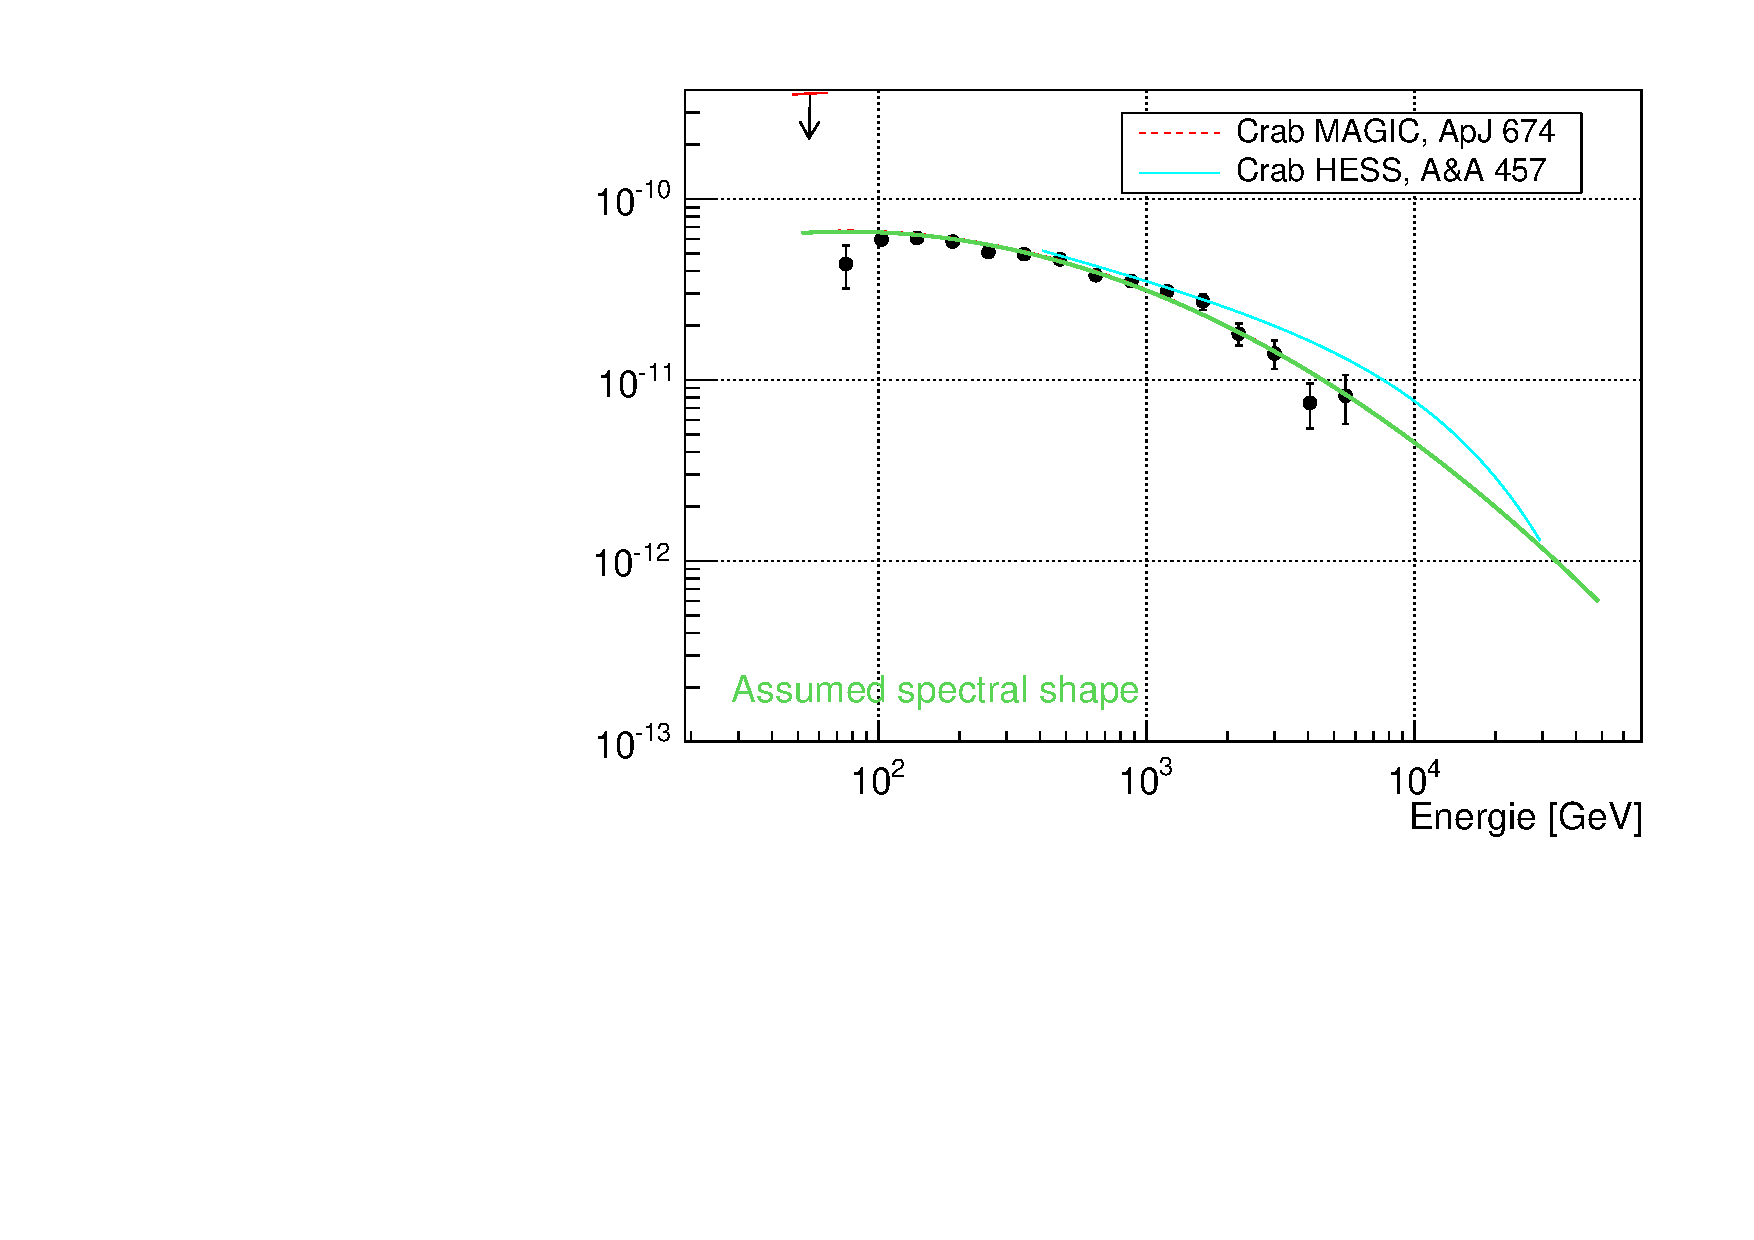
\includegraphics[width=\textwidth]{./Plots/04_MrkAnalyse/Datenset2/SED.pdf}
  \caption{SED}
  \label{Datenset2_SED_Crab}
  \end{subfigure}
  \hfill
  %-----------------------------Figure 4--------------------------------------------------------%
  \begin{subfigure}{0.45\linewidth}
  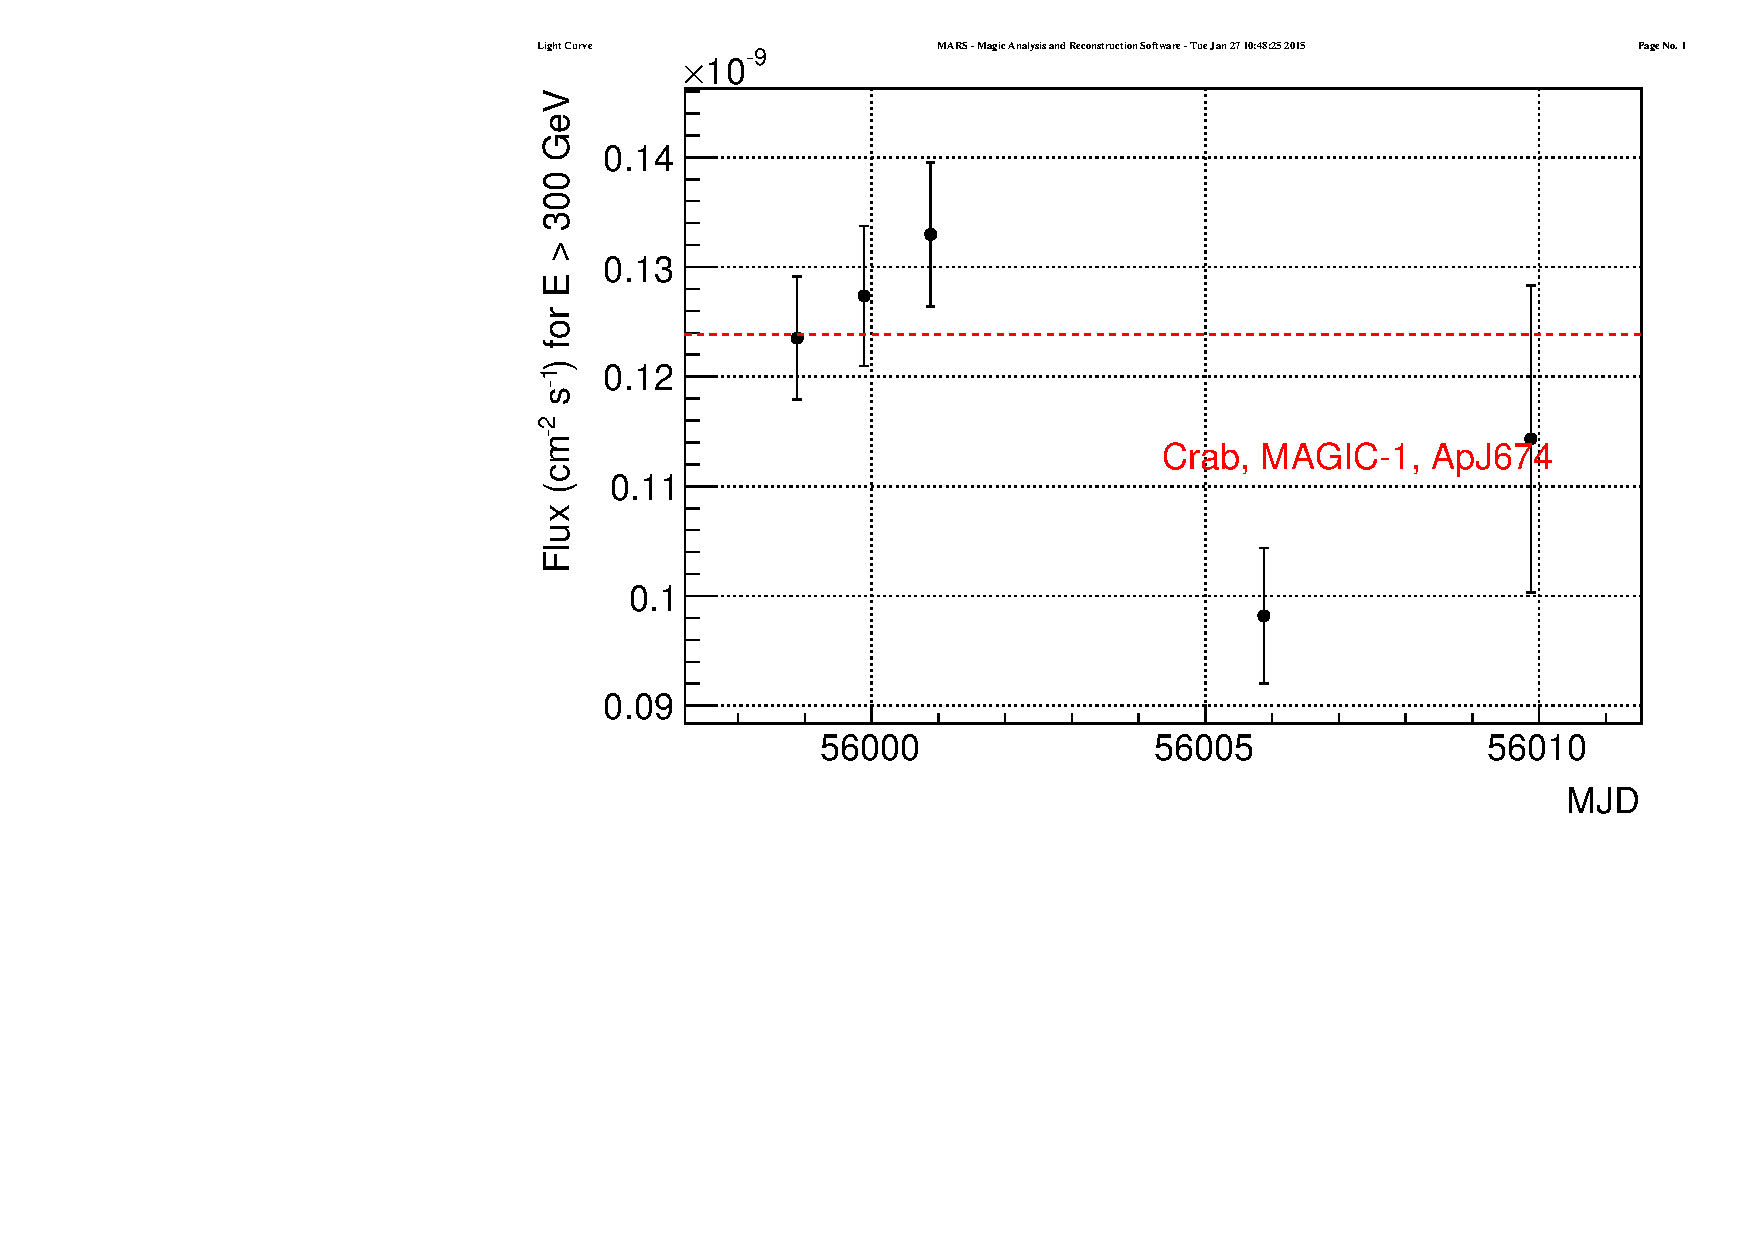
\includegraphics[width=\textwidth]{./Plots/04_MrkAnalyse/Datenset2/LC.pdf}
  \caption{Lichtkurve für Crab}
  \label{Datenset2_LC_Crab}
  \end{subfigure}
  \hfill
  %----------------------------------------------------------------------------------------------%
\caption{Flute Plots für Crab}
\label{Datenset2_Flute_Plots_Crab}
\end{figure}

In Abb.\ref{Datenset2_theta^2_Crab} ist der $\Theta^2$-Plot für Crab zu sehen, für kleine $\theta$ ist die Anzahl der Excess-Events wie zu erwarten sehr hoch.
In Abb.\ref{Datenset2_SpectralShape_Crab}, bzw in Abb.\ref{Datenset2_SED_Crab} sieht man die spektrale Energiedichte, bzw. die spektrale Energiedichte gewichtet mit $E^2$.
Wie zu sehen ist, passt das angenommene Spektrum gut zu den Daten, bzw. zum bekannten Crab-Spektrum.
Angenommen wurde folgendes Spektrum:

\begin{equation}
dN/dE=\left(\frac{x}{300}\right)^{-2.31-0.26\cdot log10(x/300.)}
 %pow(x/300.,-2.31-0.26*log10(x/300.))
\end{equation}

Die Lichtkurve in Abb.\ref{Datenset2_LC_Crab} zeigt, dass der Crab-Fluss in diesem Zeitraum um den mittleren Fluss schwankt. 

\subsubsection{Lichtkurve von Mrk421}
Es wird nun mit den gleichen Effizienz-Einstellungen wie für Crab eine Lichtkurve für Mrk421 angefertigt.

\begin{figure}
    \centering
    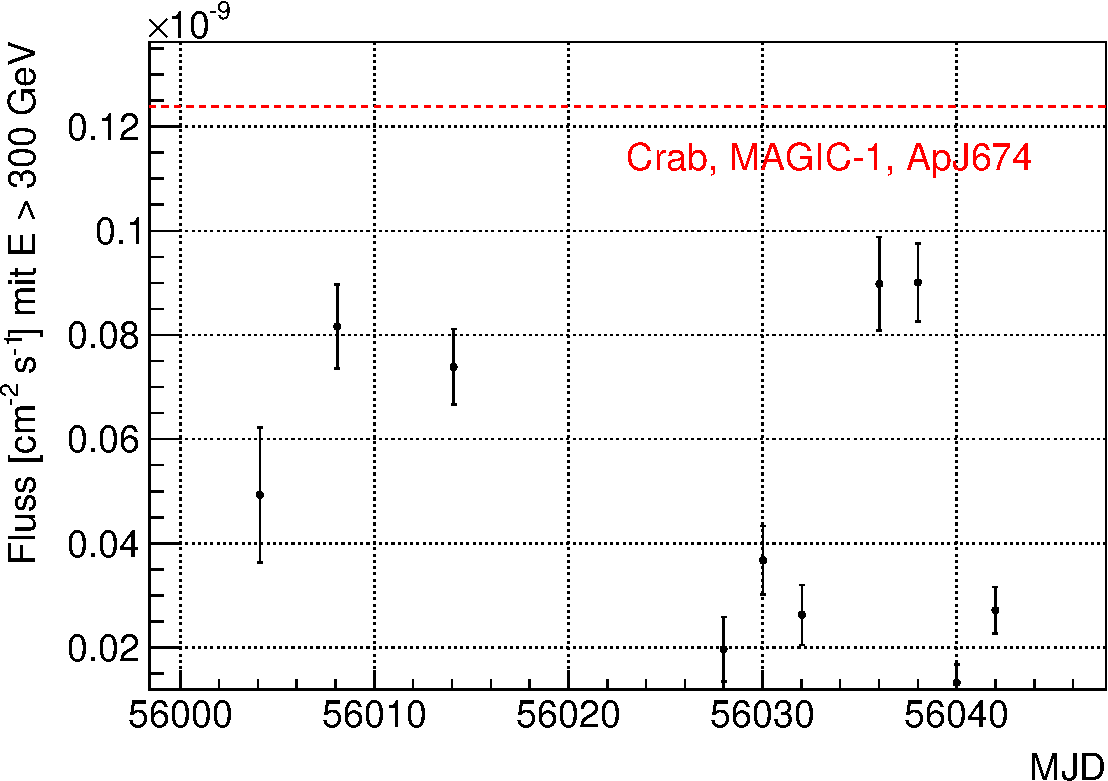
\includegraphics[width=0.8\textwidth]{./Plots/04_MrkAnalyse/Datenset2/LC_Mrk421.pdf}
    \caption{Lichtkurve von Mrk421.}
    \label{Datenset2_LC_Mrk421}
\end{figure}

Abb.\ref{Datenset2_LC_Mrk421} zeigt, dass der Fluss von Mrk421 im Vergleich zu Crab wesentlich niedriger ist.
Auch die spektrale Energieverteilung sieht anders aus (vgl. Abb.\ref{Datenset2_SED_Mrk421}).

\begin{figure}
    \centering
    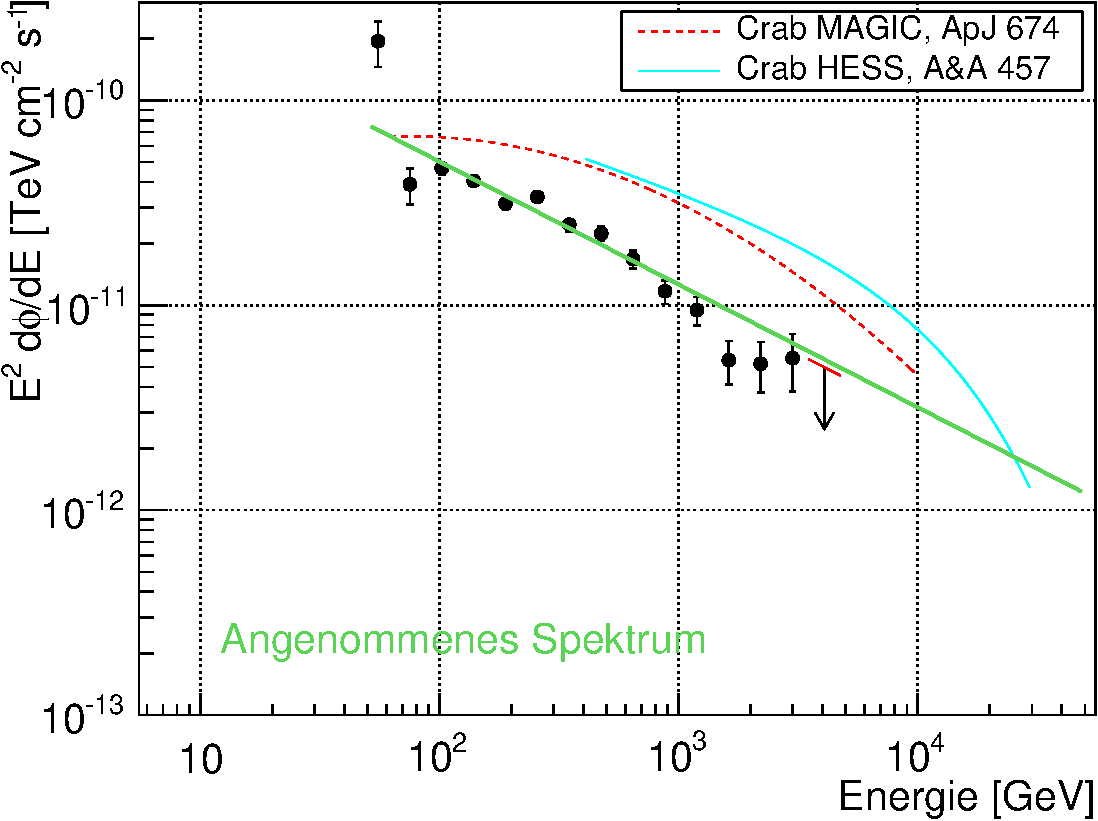
\includegraphics[width=0.8\textwidth]{./Plots/04_MrkAnalyse/Datenset2/SED_Mrk421.pdf}
    \caption{SED von Mrk421.}
    \label{Datenset2_SED_Mrk421}
\end{figure}


\subsubsection{Spektrum von Crab}
Abb.\ref{Datenset2_CombunFold_Crab} zeigt das entfaltet Spektrum von Crab mit Literaturwert.

\begin{figure}
    \centering
    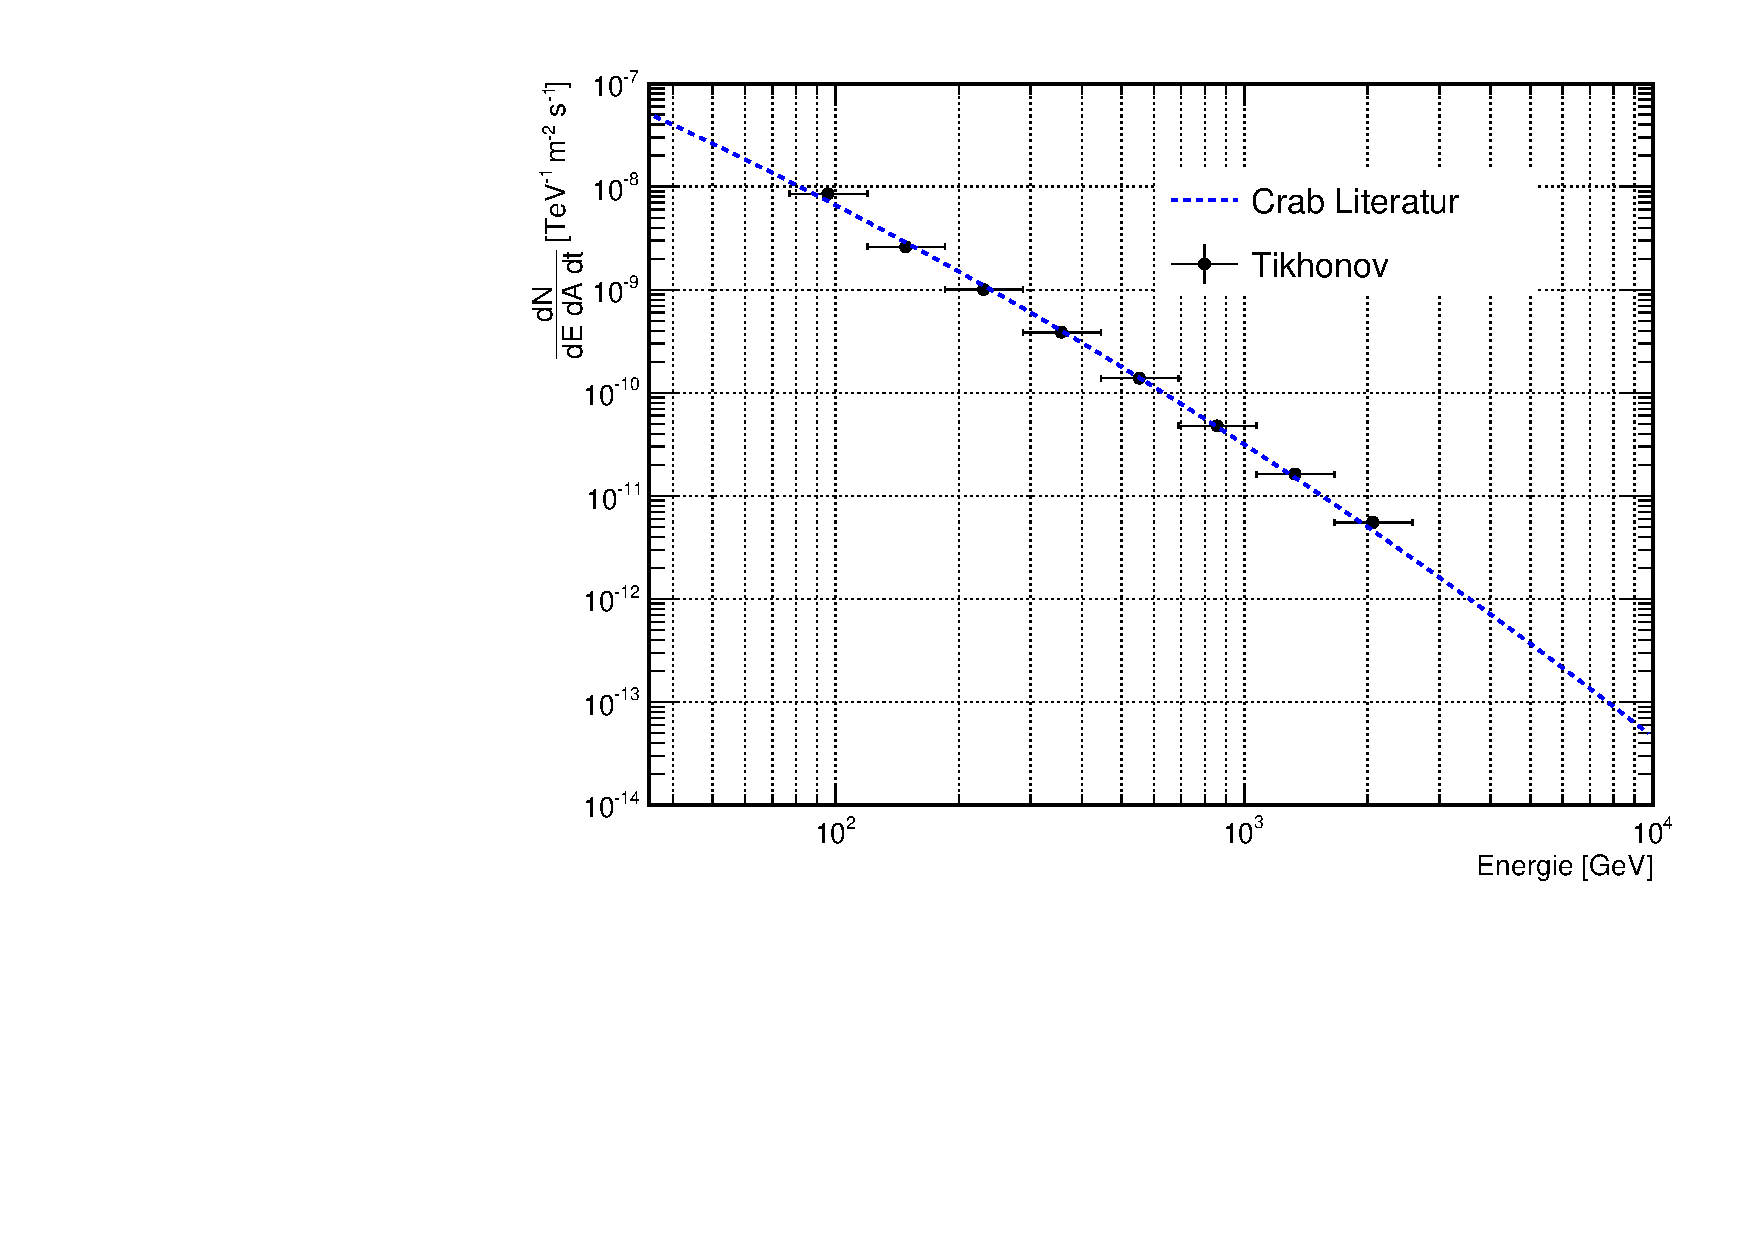
\includegraphics[width=0.8\textwidth]{./Plots/04_MrkAnalyse/Datenset2/Crab_mit_Literatur.pdf}
    \caption{Entfaltetes Crab-Spektrum mit Literatur.}
    \label{Datenset2_CombunFold_Crab}
\end{figure}


\subsubsection{Spektrum von Mrk421}
Abb.\ref{Datenset2_CombunFold_Mrk421} zeigt das entfaltet Spektrum von Mrk421 mit 5 verschiedenen Regularisierungssorten.

\begin{figure}
    \centering
    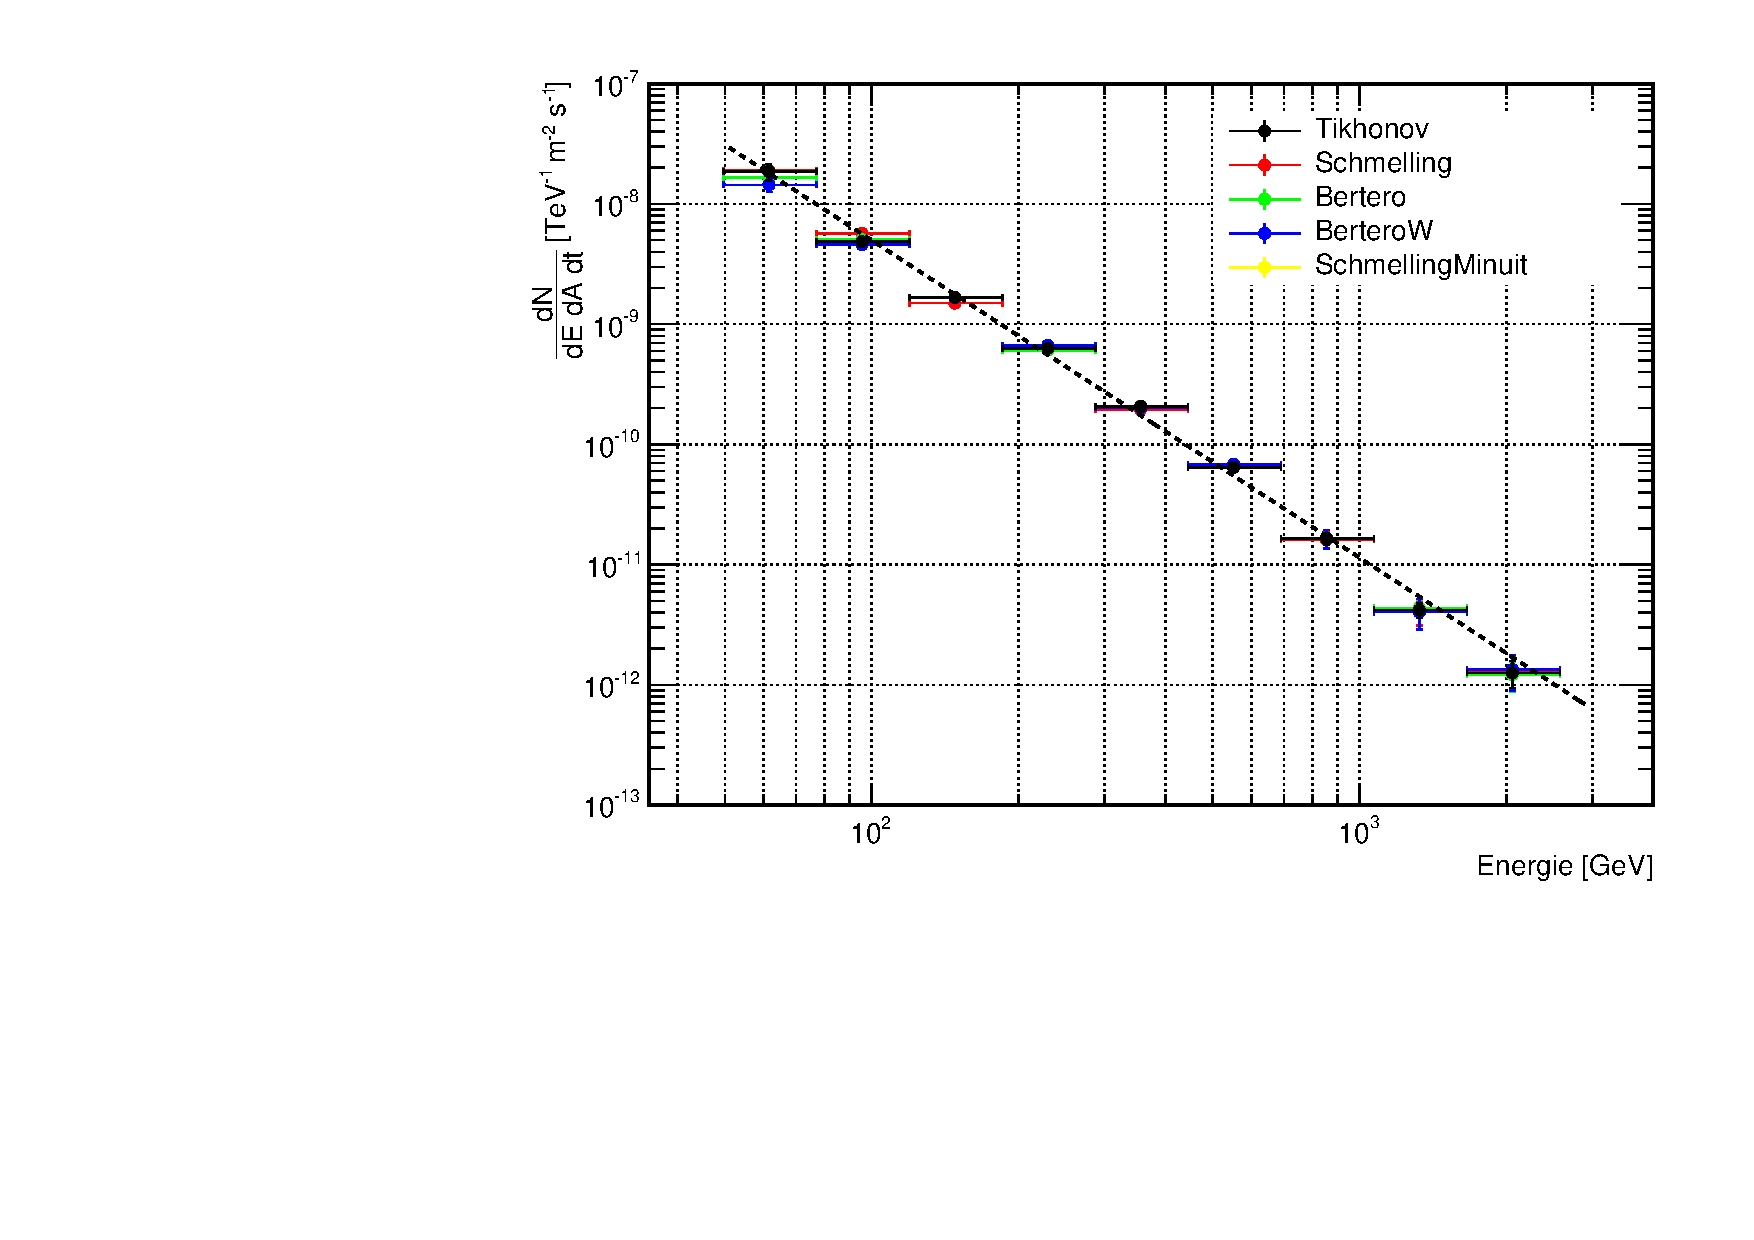
\includegraphics[width=0.8\textwidth]{./Plots/04_MrkAnalyse/Datenset2/Spektrum_Mrk421.pdf}
    \caption{Entfaltetes Mrk-Spektrum mit allen möglichen Regularisierungssorten}
    \label{Datenset2_CombunFold_Mrk421}
\end{figure}


\subsection{Teil2.1}

\subsection{Teil23}
